\documentclass[11pt,a4paper]{report}

\usepackage[T1]{fontenc}
\usepackage[utf8]{inputenc}
\usepackage[english]{babel}
\usepackage{lmodern}
%\usepackage{circuitikz}
\usepackage{color}
\usepackage{wrapfig}
\usepackage{placeins}
\usepackage{subfigure}
\usepackage{tabu}
\usepackage{fullpage}
\usepackage[squaren]{SIunits}
\usepackage{graphicx}
%\usepackage[pdftex]{graphicx}
\usepackage{epstopdf}
\usepackage{epsfig}
\usepackage{hyperref}
\usepackage{tikz}
\usepackage{tikz-qtree}
\usepackage{eurosym}
%\usepackage{chemist}
\usepackage{amsmath}
\usepackage{amssymb}
\usepackage{mathrsfs}
\usepackage{dsfont}% use $\mathds{1}$
\newcommand{\C}{\mathbb{C}}
\newcommand{\N}{\mathbb{N}}
\newcommand{\Z}{\mathbb{Z}}
\newcommand{\R}{\mathbb{R}}
\newcommand{\red}{\textcolor{red}}
\newcommand{\dis}{\displaystyle}
\newcommand{\dr}{\partial}
\newcommand{\txt}{\text}
\newcommand{\td}{\todo[inline]}
\newcommand{\ttt}{\texttt}
\newcommand{\itt}{\textit}

\usepackage{algorithm}
\usepackage{todonotes}
\usepackage[noend]{algpseudocode}

%\newtheorem{theoreme}			     {Théorème}	[chapter]
%\newtheorem{proposition}[theoreme]	 {Proposition}	
%\newtheorem{corollaire}	  [theoreme]	 {Corollaire}	
%\newtheorem{lemme}	      [theoreme]  {Lemme}		
%\newtheorem{definition}	         {Définition}[chapter]
%\theoremstyle{definition}
%\newtheorem{exemple}			     {Exemple}	[chapter]
%\newtheorem{contreexemple}[exemple]{Contre-exemple}
%\newtheorem{probleme}	             {Probl\`eme}[chapter]

\usepackage{listings}
\usepackage{textcomp}
\definecolor{listinggray}{gray}{0.9}
\definecolor{lbcolor}{rgb}{0.9,0.9,0.9}
\lstset{
	backgroundcolor=\color{lbcolor},
	tabsize=4,
	rulecolor=,
	language=matlab,
        basicstyle=\scriptsize,
        upquote=true,
        aboveskip={1.5\baselineskip},
        columns=fixed,
        showstringspaces=false,
        extendedchars=true,
        breaklines=true,
        prebreak = \raisebox{0ex}[0ex][0ex]{\ensuremath{\hookleftarrow}},
        frame=single,
        showtabs=false,
        showspaces=false,
        showstringspaces=false,
        identifierstyle=\ttfamily,
        keywordstyle=\color[rgb]{0,0,1},
        commentstyle=\color[rgb]{0.133,0.545,0.133},
        stringstyle=\color[rgb]{0.627,0.126,0.941},
}

\DeclareMathOperator{\e}{e}

\title{Titre}
\author{Florentin Goyens}
\date{\today}

\begin{document}
\tabulinesep=1.2mm
\begin{center}
\hrule
\begin{tabular}{c}
\\[0.005cm]
\Large{Applied Numerical Methods - Lab 4}\\[0.3cm]
\textsc{Goyens} Florentin  \& \textsc{Weicker} David\\[0.2cm]
$\text{6}^{\text{th}}$ November 2015\\[0.2cm]
\end{tabular}
\hrule
\end{center}


\section*{Partial differential equation of parabolic type}




\subsection*{a) Reformulation of the problem}

We apply the change of variable $T=T_{0}u$, $x=L\xi$ and $t=t_{p}\tau$. This gives 
$$\dfrac{\partial T}{\partial t } = \dfrac{\partial T}{\partial \tau }\dfrac{\partial \tau}{\partial t }= \dfrac{T_0}{t_p}\dfrac{\partial u}{\partial \tau },$$
and similarly 
$$\dfrac{\partial T}{\partial x}=\dfrac{\partial T}{\partial \xi}\dfrac{\partial \xi}{\partial x}=\dfrac{T_0}{L}\dfrac{\partial u}{\partial \xi}.$$
So we find
$$
\dfrac{\partial^2 T}{\partial x^2} = \dfrac{\partial }{\partial x}\Big(\dfrac{\partial T}{\partial x}\Big)
= \dfrac{\partial }{\partial x}\Big(\dfrac{T_0}{L}\dfrac{\partial u}{\partial \xi}\Big)
=\dfrac{\partial }{\partial \xi}\Big(\dfrac{T_0}{L}\dfrac{\partial u}{\partial \xi}\Big)\dfrac{\partial \xi}{\partial x}
=\dfrac{T_0}{L^2} \dfrac{\partial^2 u}{\partial \xi^2}.$$
The equations then becomes 
$$\rho C_p \dfrac{T_0}{t_p}\dfrac{\partial u}{\partial \tau } = k \dfrac{T_0}{L^2} \dfrac{\partial^2 u}{\partial \xi^2 }.$$
The boundary conditions on $u$ are clearly what we want using the definition of the change of variable.
$$u(0,\tau) = \left\{ \begin{array}{ll}
1, & 0\leq \tau \leq 1 \\
0, & \tau > 1.
\end{array}\right.$$ ensures that $u(0,\tau)=1$ for $0\leq \tau \leq 1$ which is gives $T(0,t)=T_0$ for the range $0\leq t \leq t_p$. We also have $T(0,t)=0$ for $t>t_p$.
The right condition $\dfrac{\partial u}{\partial \xi }(1,\tau)=0$ gives $\dfrac{L}{T_0}\dfrac{\partial T}{\partial x }(L,t)=0$. Finally the initial condition $u(\xi,0)=0$ for $0<\xi \leq 1$ is equivalent to $T(x,0)=0$ for $0<x\leq L$.\newline
For the last part of the question, writing 
$$ \dfrac{\partial u}{\partial \tau } = \underbrace{\dfrac{t_p k}{\rho C_p L^2}}_{a} \dfrac{\partial^2 u}{\partial \xi^2 }.$$
We have $a=\dfrac{t_p k}{\rho C_p L^2}$ and we check that it has no dimension. Indeed,  $$\dfrac{s \cdot J/(m \cdot s \cdot C) }{kg/m^3 \cdot J/(kg \cdot C) \cdot m^2}=
\dfrac{s \cdot J \cdot m^3 \cdot kg \cdot C}{m \cdot s \cdot C \cdot kg \cdot J \cdot m^2} $$ which simplifies.








  


\subsection*{b) Discretize to a system of equation}

Points go from $\xi_{0}=0$ to $\xi_N=1$ and there is a ghost point at $\xi_{N+1}$. The boundary condition gives the value of $U_0$ for all $\tau$ and this does not need to be an unknown of the problem we solve. The right boundary condition is $\dfrac{\partial u}{\partial \xi}=0$. We approximate with $(U_{N+1}-U_{N-1})/2h = 0$ or $U_{N+1}=U_{N-1}$. And this allows to get rid of $U_{N+1}$ and work with $U_{1}, .., U_{N}$ as the $N$ unknowns.

The equation itself is discretized to

$$\dfrac{du}{dt}(1)= \dfrac{U_{2}-2U_{1}+u(0,\tau)}{h^2}$$

$$\dfrac{du}{dt}(2:end-1)= \dfrac{U_{i+1}-2U_{i}+U_{i-1}}{h^2} \text{ for } i= 2, .., N-1.$$
$$\dfrac{du}{dt}(end)= \dfrac{2U_{N-1}-2U_{N}}{h^2} \text{ using } U_{N+1}=U_{N-1}.$$



$$\dfrac{du}{dt}= \dfrac{1}{h^2}
\underbrace{
\begin{pmatrix}
-2  & 1 &        &         &  & \\
1 & -2 & 1 &         &  & \\
       & 1 & \ddots & \ddots  &  & \\
       &        & \ddots &         &   &    \\
	   &        &        & 1 & -2 & 1\\
	   &			&		&		  & 2 & -2
\end{pmatrix}}_{A}U + \dfrac{1}{h^2} \underbrace{\begin{pmatrix}
u(0,\tau)\\
0\\
\vdots \\
0
\end{pmatrix}}_{b(\tau)}$$

Matrix $A\in \R^{N\times N}$ and vector $b(\tau)\in \R^{N}$ as explained.



\subsection*{c) Resolution}

Let us now use Euler's explicit method to solve the equation $\dfrac{dU}{d \tau}= AU+b(\tau)$ in time. The scheme gives
\begin{align*}
U^{k+1} &= U^{k} + \Delta t\Big(\dfrac{1}{h^2}AU^{k}+\dfrac{1}{h^2}b(\tau)\Big)\\
 &= \Big( I_{N} + \dfrac{\Delta t}{h^2} A\Big)U^{k} + \dfrac{\Delta t}{h^2}\cdot b(\tau)
\end{align*}
The code is available below in \ttt{tempEE.m}.

We present a stable and an unstable solution on the figures~\ref{fig:stable}\ref{fig:unstable}.
They were obtained respectively with the calls \ttt{tempEE(10,0.005,2)} and \ttt{tempEE(10,0.0051,2)}. This corresponds to $\Delta x = 0.1$ and $\Delta t = \{0.005, 0.0051 \}$. This gives $\dfrac{\Delta t}{\Delta x^2}= \{0.5,0.51\}$. The unstable case breaks the condition $\dfrac{\Delta t}{\Delta x^2}\leq \dfrac{1}{2}$.


\begin{figure}[!h]
\centering
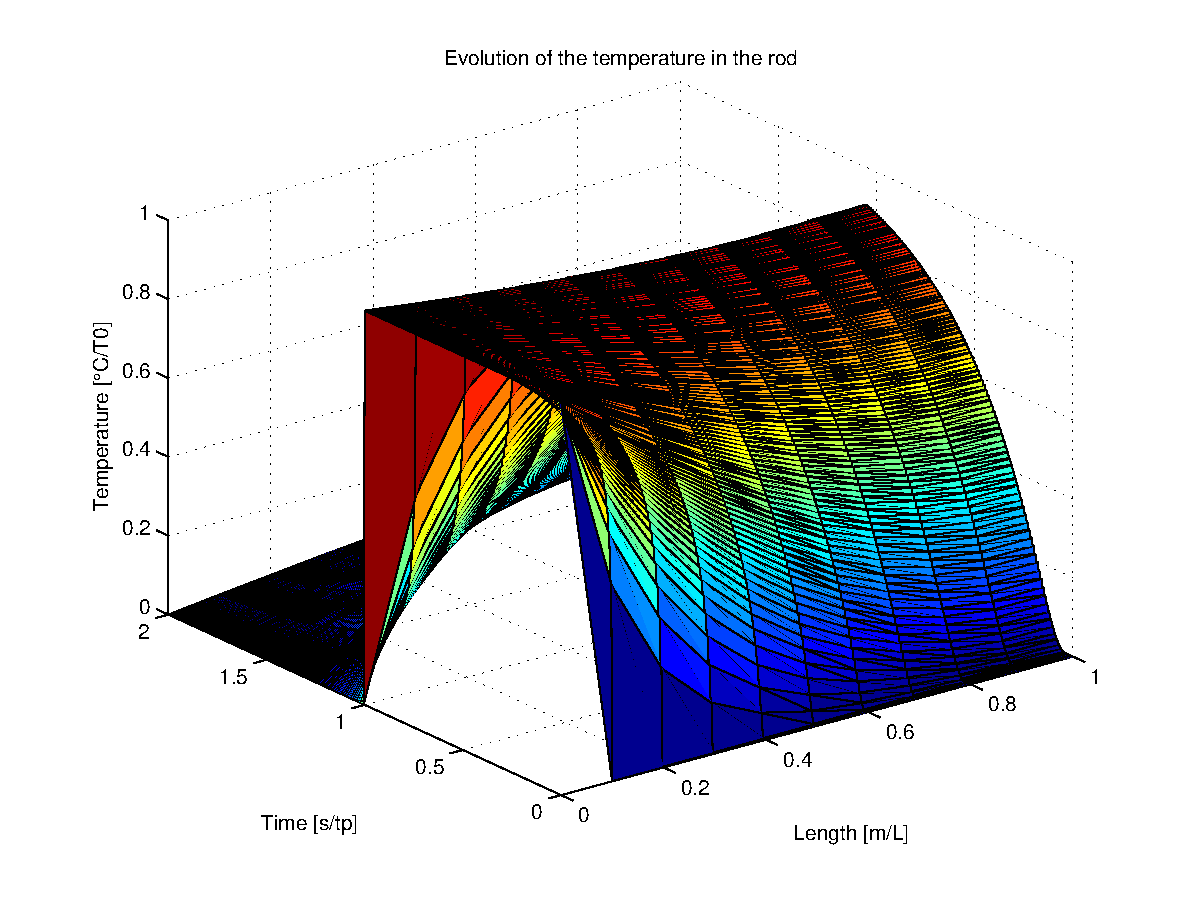
\includegraphics[width = 0.7\textwidth]{./stable.eps}
\caption{Stable solution: }
\label{fig:stable}
\end{figure}

\begin{figure}[!h]
\centering
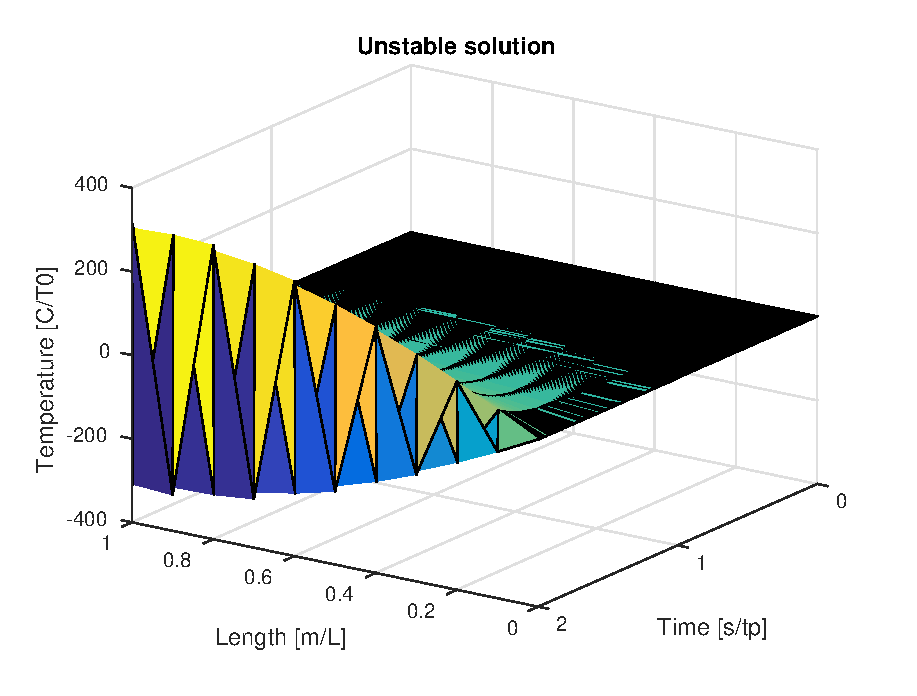
\includegraphics[width = 0.7\textwidth]{./unstable.eps}
\caption{Unstable solution: }
\label{fig:unstable}
\end{figure}
\FloatBarrier


\subsection*{d) Comparison of methods}

bla bla bla

Ceci est la partie d

\subsection*{e) Improvements}

Ceci est la partie e

\subsection*{f) Visualization}

This section is about the visualization of the results. The Matlab code can be found at the end of the report. Figure \ref{four} shows the temperature in the rod at four time points (namely $\tau \approx 0.5,1,1.5,2$).

\begin{figure}
\begin{center}
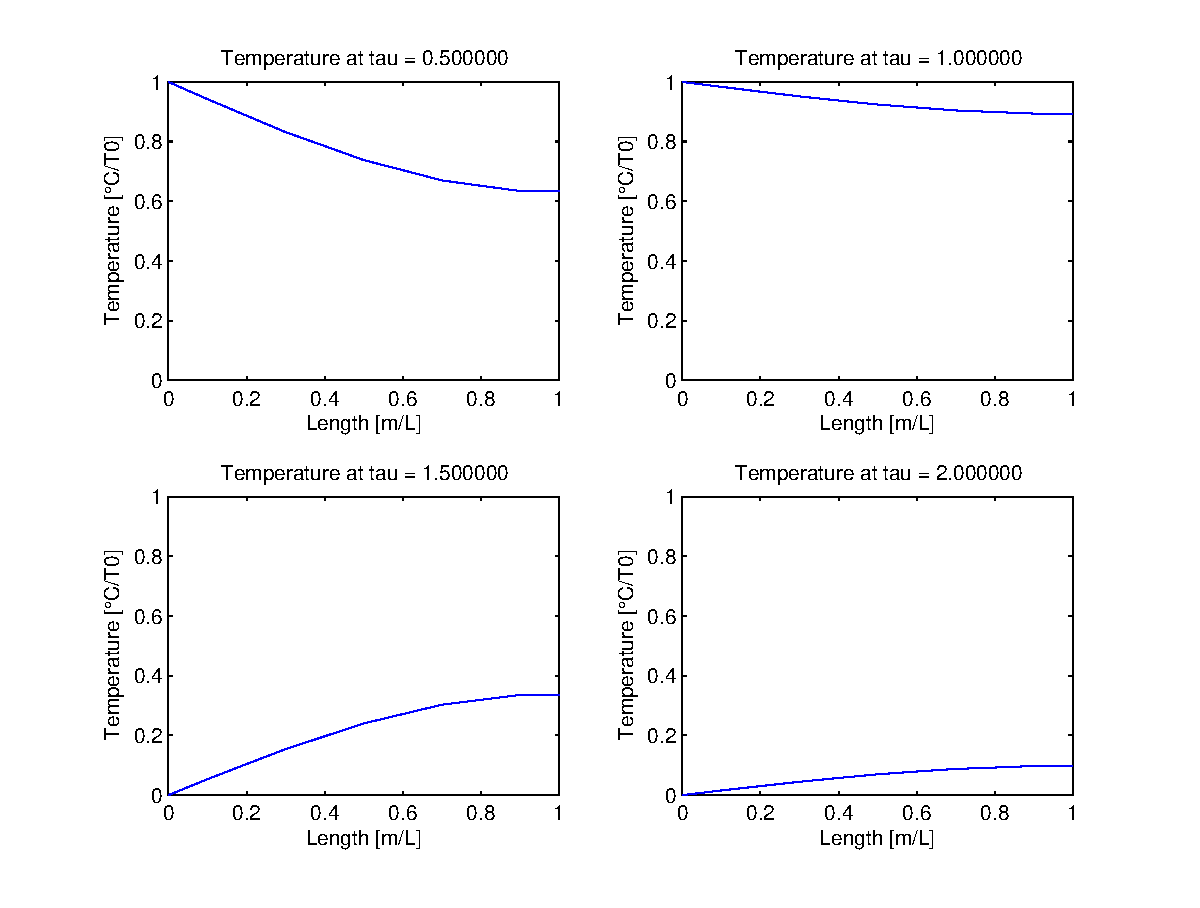
\includegraphics[width=0.9\textwidth]{four.eps}
\caption{Temperature in the rod at different times}
\label{four}
\end{center}
\end{figure}

We can notice that the boundary condition is fulfilled (as it always should be). The temperature rises until $\tau = 1$ and then starts decreasing, as it is expected. 

The next plot is the same as the stable one in section c). It is shown in figure \ref{stable}. This plot clearly depicts the boundary condition. As for the initial condition, the discretization of the $x$-axis has made it less obvious. We have in fact $u(0,0)=1$ and $u(0.1,0) = U_1(0) = 0$. Between the two, it should be zero but Matlab uses a linear interpolation. We can also see here that until $\tau=1$, the temperature is rising while it is decreasing afterwards.

\begin{figure}
\begin{center}
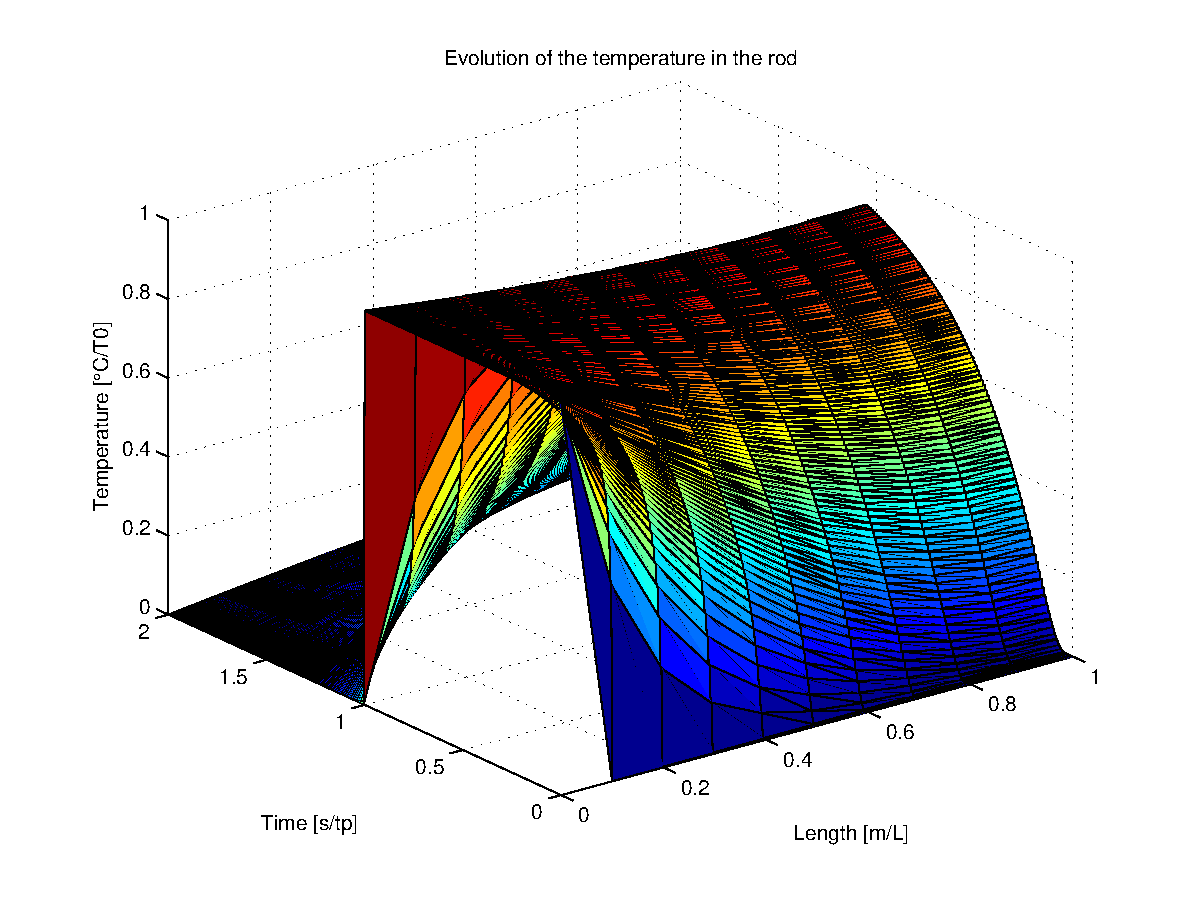
\includegraphics[width=0.7\textwidth]{stable.eps}
\caption{Temperature in the rod at any time}
\label{stable}
\end{center}
\end{figure}

\section*{Conclusion}
This report presented the solution of the very practical problem : the evolution of the temperature in a rod. This can be modelled as a parabolic PDE. To solve this PDE, we used the finite difference method to arrive at a system of ODEs. This system of ODE is stiff and a stiff method should then be used to solve it efficiently.

The stucture of the jacobian of the ODE system is really particular : it is tridiagonal (thus banded). This particularity should be taken into account when using the stiff solver (as did in section e) of the report).

\section*{MATLAB}
\lstinputlisting{graphics.m}
\lstinputlisting{tempEE.m}
\lstinputlisting{tempOde.m}


\end{document}